\documentclass[a4paper]{article}
\usepackage[pdftex]{graphicx}
\usepackage[utf8]{inputenc}
\usepackage{enumerate}
\usepackage{colortbl}
\usepackage{siunitx}
\sisetup{locale=DE} 
\usepackage{icomma}
\usepackage{amssymb}
\usepackage{tikz}
\usepackage{href-ul}
\hypersetup{
	colorlinks=true,
	linkcolor=blue,
	urlcolor=blue}
\usepackage{geometry}
\geometry{a4paper, top=15mm, left=15mm, right=15mm, bottom=15mm,
	headsep=10mm, footskip=12mm}

\begin{document}
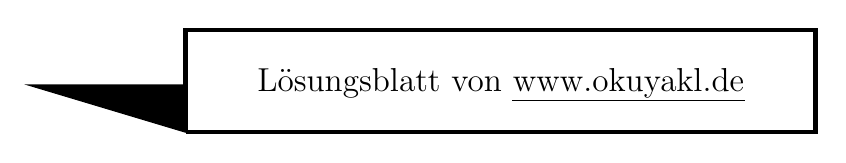
\begin{tikzpicture}(10,3)
	\draw[ultra thick](2,0) --(10,0) -- (10,1.3) --(2,1.3) -- (2,0);
	\draw[fill=black](2,0)-- (0,.6) -- (2,.6) -- (2,0);
	\node at (6,.6) {\large Lösungsblatt von \href{https://www.okuyakl.de}{www.okuyakl.de}};
\end{tikzpicture}
\vspace{0.5 cm}


\begin{enumerate}
	\item
	
\begin{enumerate}[a)]	
\item  Atome bestehen aus einem kleinen, kompakten Kern bestehend aus Protonen und Neutronen und einer im Vergleich dazu voluminösen Atomhülle, in welcher sich die Elektronen bewegen. Nahezu die gesamte Masse ist im Kern vereinigt. Gold kann man zu Folien walzen, deren Dicke nur wenige Atomlagen beträgt. Die meisten $\alpha$-Teilchen kommen beim Durchdringen dieser Folie nur mit den Atomhüllen in Kontakt, diese beeinflussen durch ihre geringe Masse deren Flugbahn kaum, denn ein $\alpha$-Teilchen, bestehend aus einem Heliumkern, ist über 5000 mal massereicher als ein Elektron. 

\item Anders sieht es aus, wenn ein solches $\alpha$-Teilchen zentral auf einen Gold-Atomkern stößt. Dieser ist deutlich schwerer als das $\alpha$-Teilchen, und wie dieses positiv geladen. Beide stoßen sich aufgrund der elektrostatischen Kraft (=Coulombkraft) ab, und das $\alpha$-Teilchen wird stark abgelenkt oder zurückgestreut.
\end{enumerate} 

\item Ein Bariumatom besteht aus 56 Protonen, die Gesamtnukleonenzahl ist 138. Hieraus errechnet sich eine Neutronenzahl von $ 138-56= 82 $. Zu jedem Proton gehört ein Elektron, also sind es ebenfalls 56 Elektronen.

\item Der 56-fach positiv geladene Kern ist umgeben von 56 Elektronen, die jeweils eine negative Ladung tragen. Die Ladungsschwerpunkte der beiden sich überlagernden elektrischen Felder fallen zusammen und neutralisieren sich in ihrer Wirkung.

\item Aufgabe 
\begin{enumerate}[a)]
	\item $$ {}^{206}_{~81}\mathbf{Tl} \qquad \Longrightarrow \qquad {}^{206}_{82}\mathbf{Pb} \qquad + \qquad {}^{~0}_{-1}\mathbf{e}$$

\item 
\renewcommand{\arraystretch}{2}
\begin{tabular}{|>{\columncolor[gray]{.8}}p{1.8 cm}|p{1.5 cm}|p{1.5 cm}|}
	\hline
	\rowcolor[gray]{.8}	Zeit in min & Masse Thallium & Masse Blei \\
	\hline
	0 & $\SI{1000}{\milli\gram}$ & $\SI{0}{\milli\gram}$\\
	\hline
	4,2 & $\SI{500}{\milli\gram}$ & $\SI{500}{\milli\gram}$\\
	\hline
	8,4& $\SI{250}{\milli\gram}$ & $\SI{750}{\milli\gram}$\\
	\hline
	12,6& $\SI{125}{\milli\gram}$ & $\SI{875}{\milli\gram}$\\
	\hline
	42& $\SI{1}{\milli\gram}$ & $\SI{999}{\milli\gram}$\\
	\hline
\end{tabular}	

\item Nein, bei einer exponentiellen Abnahme wie in diesem Fall erreicht der Funktionswert nie Null.
\end{enumerate} 

\item
Es gibt Up-Quarks mit der Ladung $ + 2/3$ und Down-Quarks mit der Ladung $ - 1/3$ Protonen bestehen
aus zwei Up- und einem Down-Quark, tragen also die Ladung $ + 2/3 + 2/3 - 1/3 = +1$; Neutronen hingegen bestehen aus zwei Down, und einem Up-Quark. Ihre Ladung ist $ + 2/3 - 1/3 - 1/3 = \pm 0$, sie sind neutral.


\item  

$\alpha$-Strahlung
\begin{itemize}
	\item besteht aus schnellen Heliumkernen.
	\item Sie ist ionisierend.
	\item Sie wird durch Papier abgeschirmt
\end{itemize}

$\beta$-Strahlung
\begin{itemize}
	\item besteht aus schnellen Elektronen.
	\item Sie ist ionisierend.
	\item Sie wird durch dünne Metallplatten abgeschirmt
\end{itemize}

$\gamma$-Strahlung
\begin{itemize}
	\item besteht aus Photonen.
	\item Sie ist ionisierend.
	\item Sie wird durch dicke Bleiplatten abgeschirmt
\end{itemize}

\item
Vor dem $\alpha$-Zerfall war die Massenzahl um vier höher, die Ordnungszahl um zwei. Im PSE finden wir an dieser Stelle Radium.
$$  {}^{222}_{~88}\mathbf{Ra} \qquad \longrightarrow \quad {}^{218}_{~86}\mathbf{Rn} \quad + \quad {}^{4}_{2}\mathbf{He} $$

\item
Es gilt das Zerfallsgesetz:
$$ A(t)=A_0 \cdot \left( {1 \over 2} \right)^{t \over T_{1/2}}$$
Hierbei ist $A(t)$ die Aktivität nach der verstrichenen Zeit $t$,
$A_0$ die Anfangsaktivität zum Zeitpunkt $t=0$ und $T_{1/2}$ die Halbwertszeit. Die verstrichene Zeit und die Halbwertszeit müssen in der gleichen Einheit eingesetzt werden. So ergibt sich:
$$  A(t)=\SI{2,5e3}{\becquerel}\cdot \left( {1 \over 2} \right)^{2020-1966 \over 29~\rm{a}}= \SI{688}{\becquerel}$$

\item
75\% sind zerfallen, wenn $1\over 4$ der ursprünglichen Menge noch vorhanden sind. Es sind also $${1\over 4} = \left({1\over 2}\right)^2$$ zwei Halbwertszeiten vergangen.
In Jahren macht dies: $$2 \cdot 29~\rm{a} = 58 ~\rm{a}$$

\item
Die Massenzahl Z ändert sich nur mit der Anzahl $n$ der $\alpha$-Zerfälle; und zwar um jeweils vier. Wir rechnen:
$$232 - 4\cdot n = 208  \qquad \Rightarrow \qquad n = 7 $$  
Nach 7 $\alpha$-Zerfällen wäre die Kernladungszahl $\tilde{A}$:
$$ \tilde{A} = 90 - 7 \cdot 2 = 76 $$
Es ist aber $ A = 82$ ; die Differenz gibt die Anzahl $m$ der $\beta$-Zerfälle, weil bei jedem $\beta$-Zerfall die Ordnungszahl um eins steigt:
$$ m = 82 - 76 = 6 $$
 
\begin{center}
	\includegraphics[width=7 cm]{../../viecher/endcomic.pdf}
	
	Hier geht es zurück zum \href{https://www.okuyakl.de/phys/p9atoL412/aa412.pdf}{Aufgabenblatt}
\end{center}

\end{enumerate}
\end{document}

